\documentclass[onecolumn, oneside, letterpaper, draftclsnofoot, 10pt, compsoc]{IEEEtran}

\usepackage[english]{babel}
\usepackage{graphicx}
\usepackage{url}
\usepackage{setspace}
\usepackage{subcaption}
\usepackage{verbatim}
\usepackage{amssymb}
\usepackage{amsmath}
\usepackage{amsthm}
\usepackage{alltt}
\usepackage{color}
\usepackage{enumitem}
\usepackage{textcomp}
\usepackage{cite}

%\usepackage[T1]{fontenc}
\usepackage[utf8]{inputenc}
\usepackage{lmodern}
\usepackage[hidelinks]{hyperref}
\usepackage[normalem]{ulem}

\usepackage[margin=0.75in]{geometry}

%\parindent = 0.0 in
%\parskip = 0.05 in

% 1. Fill in these details
\def \CapstoneTeamName{         Beaver Hawks}
\def \CapstoneTeamNumber{       14}
\def \GroupMemberOne{           Anton Synytsia}
\def \GroupMemberTwo{           Matthew Phillips}
\def \GroupMemberThree{         Shanmukh Challa}
\def \GroupMemberFour{          Nathan Tan}
\def \CapstoneProjectName{      American Helicopter Society Micro Air Vehicle Competition}
\def \CapstoneSponsorCompany{   Potentially Columbia Helicopters}
\def \CapstoneSponsorPerson{    Nancy Squires}

% 2. Uncomment the appropriate line below so that the document type works
\def \DocType{Progress Report}

\newcommand{\NameSigPair}[1]{\par
\makebox[2.75in][r]{#1} \hfil   \makebox[3.25in]{\makebox[2.25in]{\hrulefill} \hfill        \makebox[.75in]{\hrulefill}}
\par\vspace{-12pt} \textit{\tiny\noindent
\makebox[2.75in]{} \hfil        \makebox[3.25in]{\makebox[2.25in][r]{Signature} \hfill  \makebox[.75in][r]{Date}}}}
% 3. If the document is not to be signed, uncomment the RENEWcommand below
%\renewcommand{\NameSigPair}[1]{#1}

%%%%%%%%%%%%%%%%%%%%%%%%%%%%%%%%%%%%%%%
\begin{document}
\begin{titlepage}
    \pagenumbering{gobble}
    \begin{singlespace}
        %\includegraphics[height=4cm]{coe_v_spot1}
        \hfill
        % 4. If you have a logo, use this includegraphics command to put it on the coversheet.
        \begin{center}
        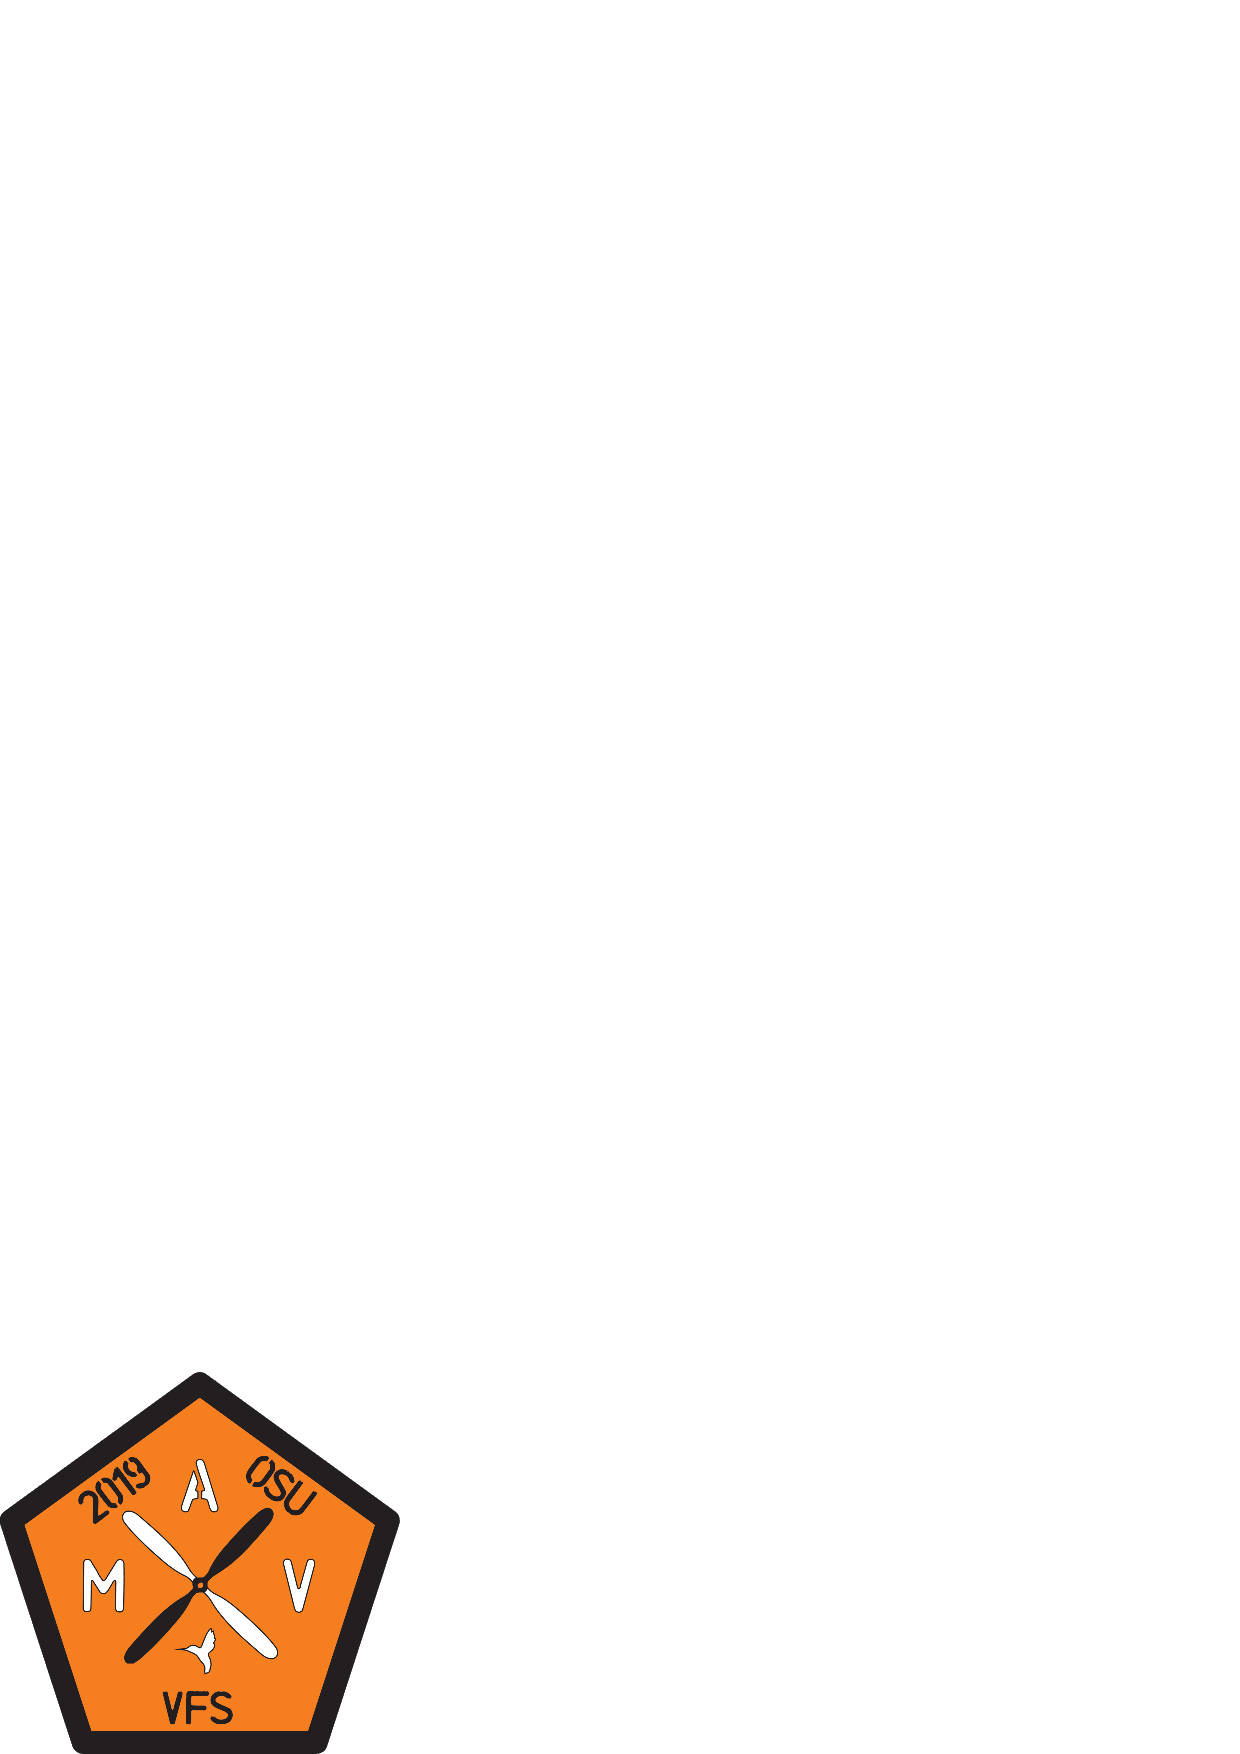
\includegraphics[height=4cm]{graphics/logo.png}
        \end{center}
        \par\vspace{.2in}
        \centering
        \scshape{
            \huge CS Capstone \DocType \par
            {\large\today}\par
            \vspace{.5in}
            \textbf{\Huge\CapstoneProjectName}\par
            \vfill
            {\large Prepared for}\par
            \Huge \CapstoneSponsorCompany\par
            \vspace{5pt}
            {\Large\NameSigPair{\CapstoneSponsorPerson}\par}
            {\large Prepared by }\par
            Group\CapstoneTeamNumber\par
            % 5. comment out the line below this one if you do not wish to name your team
            \CapstoneTeamName\par
            \vspace{5pt}
            {\Large
                \NameSigPair{\GroupMemberOne}\par
                \NameSigPair{\GroupMemberTwo}\par
                \NameSigPair{\GroupMemberThree}\par
                \NameSigPair{\GroupMemberFour}\par
            }
            \vspace{20pt}
        }
        \begin{abstract}
        \end{abstract}
    \end{singlespace}
\end{titlepage}
\newpage
\pagenumbering{arabic}
\tableofcontents
% 7. uncomment this (if applicable). Consider adding a page break.
%\listoffigures
%\listoftables
\clearpage

\section{Project Purpose}
% Talk about VFS and why they host competition
The Vertical Flight Society is the world's premiere international technical society for engineers, scientists and others working to advance vertical flight. VFS brings together industry, academia and government to face difficult challenges in vertical flight. Each year, VFS hosts the Micro Air Vehicle challenge to help prepare and attract the next generation of scientist and engineers to work in the field of vertical flight.


\section{Project Goals}
The goal of this project is to collaborate closely with the mechanical engineering and electrical engineering subteams in building a micro air vehicle to accomplish the mission presented by the Vertical Flight Society.

% Anton
\subsection{Challenge Details}
\noindent
The mission is to have a micro air vehicle complete an obstacle course, themed as Washington’s Flight for Liberty. The competition, to be held in Philadelphia, is comprised of an obstacle course map, as displayed in the current slide. The obstacle course is to be completed in under a ten minute time limit. A grade is assigned based on the performance and reliability of completed tasks. Step-by-step objectives, include:

\begin{itemize}
    \item Take of from Thomas Paine\textquotesingle s helipad and acquire the package.
    \item Fly over a six foot net barrier and head north until reached McKonkey\textquotesingle s Ferry.
    \item Cross the Delaware River and release the package at Pamphlet Delivery helipad.
    \item Make way to Camp Washington, flying south over a four foot obstacle and under a two foot barrier.
    \item Acquire a different package at Camp Washington and return all the way back to Thomas Paine\textquotesingle s helipad, following the same route.
\end{itemize}

\noindent
With the challenge described, we will now talk about our team\textquotesingle s objective, specifically.

% Anton
\subsection{Objective}
\noindent
Computer science team\textquotesingle s objective is to develop a graphical user interface for the pilot to rely on during the Vertical Flight Society\textquotesingle s Micro Air Vehicle challenge. Mandatory components include video feed from front a facing camera. We, however, intend to take our user interface much further than just displaying the front video feed. Planned features include bottom camera feed, package pickup assist, collision warning, attitude indicator, velocity indicator, and height indicator. We also intend to expand computer science influence to on-board the helicopter. On-board components include collision avoidance, LED control, and speaker control. Each of these features are describes in the following sections.


\section{Project Development}
% Briefly outline all the documents we wrote
% Nathan
\noindent
So far for this project, we have written a lot of documentation in preparation for the development of the project. These documents include a problem statement, a requirements document, a technology review, a design document, and finally, this progress report.
\subsection{Problem Statement}
\noindent
The problem statement helps to define the scope of our project. It introduces important definitions that help to define what our project is about and why we are doing this project. A big part of this document is defining abilities that our helicopter needs to have to complete the obstacle course and do well in the competition.
\subsection{Requirements}
\noindent
The requirements document outlines the technical scope of our project. It defines terms that are important for understanding the technical aspects of the desired outcome for our helicopter\textquotesingle s build and functionality. Also outlined in the requirements document are the specific rules for the competition, including the obstacle course layout, helicopter build limitations, designated flight path, key landmark descriptions, and payload descriptions.
\subsection{Technology Review}
\noindent
% Why we wrote tech reviews, but do not mention your tech
Each member of our team conducted separate technology reviews that each consisted of three technology topics relevant to deciding what technology to use when developing the helicopter. There was a bit of overlap in the technology review topics, but together all the necessary technologies were covered. Our technology reviews covered hardware components mounted on the helicopter, software libraries for on-board the helicopter, and software for sending and displaying the helicopters camera feed to the pilot. By researching different technologies and documenting them, we made informed decisions about how to design the best helicopter for the competition in terms of software.
\subsection{Design}
The purpose of the design document is to flesh out all the components that will be implemented. The document provides details for the structure of two main bodies of software, the software running on the Raspberry Pi Zero, which operates the helicopter to an extent, and the software on the laptop which will be responsible for receiving transmitted data and presenting it to the pilot in a helpful fashion.
\noindent


\section{Problems and Solutions}
\subsection{Hardware Limitation}
% Hardware limitations
% Our hardware needs to fit weight limit
% Camera needs to be high resolution and be compatible with Raspberry Pi, be X frames per second
The biggest constraint on the project is the weight limit of the vehicle. Since there is a 500 gram limit on total vehicle weight, our team could not have everything we wanted. Initially, we wanted to have an Intel Realsense camera on the front of the helicopter. This would have been great for the competition because the Realsense camera provides object detection and relative distances for each object. Also, Intel provides software packages to use with their hardware, making development using the Realsense camera much easier. Unfortunately, the Realsense camera uses a USB-C style connector. The USB-C style connector is not used on Raspberry PIs or Arduino boards, and systems that support USB-C are too heavy for the helicopter. The weight limit prevented our use of the Intel Realsense.

\noindent
Next we thought to use a system of infrared lasers and an infrared camera as a range finding system. By measuring pixel distances of the infrared lasers detected by the infrared camera, we could determine how far away an object is. This system had the advantage of being cheap and light weight, but also the disadvantage of having not software packages available for use, meaning everything need would need to be coded from scratch.

\noindent
Fortunately, we found another system that fit our requirements much better. The Eys3D camera is a stereographic infrared camera system. The Eys3D system does not provide object recognition, but it does provide a color video feed and a depth map of the current camera view area. Also, it is light weight and uses a micro USB style connector.

\noindent
We also faced other minor challenges, like needing to purchase more expensive ultrasonic sensors because cheap ultrasonic sensors are heavy.
\subsection{Team Collaboration}
% Team collaboration
% Talk about how we convinced ECE and ME teams to include our design component
We faced probably the same problem that most large teams face: coordination of effort. The complete team is 23 memembers and trying to schedule a meeting time for 23 different people is very challenging.
Another challenge for the large team was unifing the team's vision of the helicopter. The MEs and the CSs initially had very different ideas about the CSs' role in the project. However, the CS team's persistence and persuasiveness paid off, and we convinced the team of the value of our contributions to the project which led to changes in the planned implementation of the onboard hardware. Specifically, we convinced the team of the need for a more powerful onboard processor and the benefits of having a camera with the capability of depth mapping.

\noindent
On the CS team level, we had a hard time during the run up to finals week. We were so busy that meeting and working together on the project was near impossible.

\section{Project Design}
% Project Design Details and Tech Review ?
% Nathan
As our project currently stands, in addition to the written documentation, we have designed a software architecture for our teams helicopter. This design takes into account a range of sensors and two cameras. Our design takes in this data on-board the Raspberry Pi, and sends the data to the appropriate place, whether that means it is sent back to the computer, or it is also used on-board the Raspberry Pi.


\subsection{Front and Bottom Video Feed}
% Nathan
A big part of this project for the Computer Science team is to deal with the cameras on the MAV. There are specific portions of the obstacle course where the pilot will have not have sight of the MAV. For these parts of the course, we have a front facing camera that allows the pilot to make important decisions when piloting the MAV. The MAV design has an additional downward facing camera to assist with package pick-up. These camera feeds by design will be sent to a server run locally on a laptop, where the same laptop will display a view containing these feeds for the pilot\textquotesingle s viewing.


\subsection{Package Guidance}
% Shanmukh
% Mention bottom facing camera, image recognition. Talk about GUI and details in current project state section.
Another major aspect of the remote-controlled helicopter is the payload pickup assistance. To accomplish this, we will be using a bottom facing camera to obtain a video feed and will use computer vision to navigate the pilot to an optimal pickup point. With the other major requirements needed to successfully compete in the competition, such as the front-facing cameras and sensors, we are classifying this as a stretch goal.

\noindent
Computer Vision is an essential portion of this segment to enable the pilot to view and detect obstacles that may appear in its path. The American Helicopter Society competition contains a course with obstacles such as walls, trees, and bridges. Additionally, a part of the course cannot be seen through human eyes, so the helicopter must solely rely on a camera. Computer Vision will allow the pilot to have other intelligence data that can assist in avoiding obstacles, and reach the appropriate pickup or drop off point. If we decide to build this feature, our team will use OpenCV because of the real-time image recognition benefits and it is a low-cost option.

\noindent
OpenCV has various inbuilt functions that allow a user to inference objects and perform actions quickly. Since OpenCV is a software development kit, the inferencing and machine learning must be performed on the local machine as there is no cloud option available. Additionally, OpenCV allows us to detect and recognize objects in real-time, so it is the chosen API for our product. Specifically, we will be using OpenCV on the bottom-facing camera to find an optimal pickup point for the payload. The general workflow we will be using to leverage machine learning methods to navigate the pilot to this optimal pickup point is as follows:

\noindent
Each of the components performs a significant task in developing an intelligent platform to detect the pickup points.
\begin{itemize}
    \item Training Data: Gather image data of the payload pickup and drop-off point based on the competition information.
    \item Data Preprocessing: Before data, the data needed to be cleaned to a unified structure that allows for equal learning opportunities to learn.
    \item Training: Training the image data is a critical portion of image recognition. The training segment is where the machine learns to distinguish between different objects.
    \begin{itemize}
        \item Neural Network: The current design choice is to build a neural network, which is a deep learning mechanism to train our model. While computationally expensive, a neural network generally yields accurate results when inferencing an object.
    \end{itemize}
    \item Output Weights File: The weights file is the multidimensional output from the training. It is the neural network connections that were generated in order to achieve accurate inferencing.
    \item Using Weight file for object recognition: Once the weight file is ready from the training, we load the file into the computer vision application which enables the inferencing.
    \item Decision: Finally, the local machine has the ability to detect objects in real-time (in this scenario, we now have the ability to find an optimal payload pickup point).
\end{itemize}

\noindent
The video feed of the computer vision application will be displayed on the Graphical User Interface (GUI) will be discussed later.

\noindent
After talking amongst our team and other sub-teams, we feel that this computer vision application for the bottom-facing camera could assist the pilot while picking up the package. In the previous years, payload pickup was a challenging component of the competition. Teams often lose the most time when picking up and dropping off a package because they are unable to find an efficient point to disembark and load the package. The machine learning technology onboard is intended to help the pilot navigate to a position which is easiest for pickup.

\subsection{Collision Warning}
% Anton
In addition to providing the pilot with video feed and package retrieval guidance, our design includes a collision warning system. The collision warning system provides the pilot with awareness of the surrounding obstacles, beyond the field of view provided by the front camera. The system works in the following way. Three LV-MaxSonar ultrasonic range sensors supply the interface with an instantaneous feed of obstacle detection ranges. The ranges are converted to a color scheme, ranging from green, being the farthest, to red, being the nearest. The colors are then applied to their associated semi-pie graphical user interface elements, shown in the slide. Because the pilot is not expected to look at the screen, a beeping warning sound is echoed whenever obstacles penetrate a safe radius.

\noindent
One of the natural things the collision warning interface provides is the ability for the pilot to position the aircraft in a tight space with obstacles. For example, whenever performing a flight through a tunnel, the pilot can focus on balancing the left and right colors within the GUI, in turn for equalizing the distances to left and right walls.

\noindent
Due to potential battery power and vehicle mass limitations, our current design does not include a sensor for the rear view of the micro air vehicle. If, however, the electrical and computer engineering team, as well as the mechanical engineering team, determines that power and mass can be allocated, additional ultrasonic range sensor will be included. In the meantime, we assume the pilot restricts their maneuverability to forward and sideways.

\subsection{Collision Avoidance}
% Anton
Our stretch goal is to include collision avoidance system, where remote controls are overridden to keep the MAV at a safe distance from the obstacles. Collision avoidance is collision warning at the next level. Whenever the MAV is too close to an obstacle, the collision avoidance system overrides controls to prevent the MAV from moving further toward the obstacle. Additionally, the collision avoidance computes proper rejection pitch and roll components to ensure that the MAV does not keep moving in the direction of an obstacle.

\noindent
Collision avoidance involves all the range sensors, accelerometer, and potentially the depth map from the front facing camera. For rapid response, collision avoidance is processed onboard the MAV. Displayed in the figure is a mock up how pitch and roll controls are to be overridden.

\subsection{Flight Instruments}
% Matthew
% Attidute indicator, speed indicator, height detection
% Refer to design document for details on these instruments
There are two variables used to stabilize the helicopter. The accelerometer detects magnitude and the direction of movement and the gyroscope tracks the orientation of the vehicle. These variables are fed into the helicopter's onboard computer which calculates the proper values for the helicopter’s pitch, roll, collective pitch, torque, and throttle. Stable hover and stable flight are achievable because of the onboard accelerometer and gyroscope.

\noindent
The third flight variable is height. Height is not directly used in stabilizing the craft, but is used for assisting with package pickup. The height value comes from a downward facing sonic sensor. Height is used, along with image recognition software, to help the pilot pick up the target package, or if selected, automatically adjust the helicopter’s position over the target.


\section{Weekly Report}
% Throw in your weekly progress into the associated week sections.
% We will combine them later and remove redundancy

\subsection{Week 3}
%script read
\noindent \textbf{Progress}\\ \noindent
Overall, week 3 was a very busy week. Our group was assigned to a Micro Air Vehicle Challenge hosted by the vertical flight society. We met up with our other team members. There are three subteams to the whole team. The three subteams are made of CS students, ME students, and ECE students. The MEs and ECEs were already assigned to the project before us. Our first day we were introduced to last year's project and showed the helicopter from last year’s team. Initially our group used email and text messaging exclusively, however, we decided to setup a Slack channel to help our group stay organized. We also tried to start coordinating our efforts with the ECEs at the beginning because our designs interact closely.

\noindent \textbf{Problems}\\ \noindent
We also still needed to contact our client and determine our meeting times with the TA.

\noindent \textbf{Plans}\\
We decided to meet up on Friday with the ME subteam lead to discuss the project and sensors we would be interested in implementing.

%end script
\begin{comment}.
%commented out just in case we need the progress/prob/plan format later
\subsubsection{Anton's Weekly Progress}
\noindent \textbf{Progress} \newline \noindent
We have met up with one of our team members, who has already been assigned to the project before us. He introduced us to the project and showed the helicopter we will be using. We also planned a meeting time on Friday.

\noindent \textbf{Plans} \newline \noindent
We decided to meet up on Friday with the ME leader to discuss the project and sensors we would be interested in implementing. We also need to contact our client and determine the TA meeting times. We hope to accomplish this at the Friday\textquotesingle s meeting.

\subsubsection{Nathan's Weekly Progress}
\begin{itemize}
    \item Progress:

So far I have meet with my group and we have decided to communicate mainly through texting and occasionally through email. All members of the team were present and Shamukh, who has been meeting with the other subsets of the competition team, showed us the helicopter from last years competition.
    \item Problems:

Shamukh has meet with the client, Nancy, or at least that is my current understanding. But to my knowledge we have not yet designated a routine time to meet with Nancy.
    \item Plans:

October 12th will be the first time all the sub-teams will meet to discuss the project.
    \end{itemize}
\end{comment}
\subsection{Week 4}
%scripted used
\noindent \textbf{Progress}\\
From Tuesday through Thursday, we worked on and completed our group problem statement. Using the required \LaTeX\ capstone template, we submitted it on Friday. On Wednesday, at noon, we met with our TA, Ben. We asked Ben for insight on choosing the right kind of camera for recognition and parallax vision, as well as, the right type of ultrasonic range sensor. Luckily for us, Ben's thesis is on computer vision and turned out to be very skilled in the area of our project. Ben guided us toward choosing the right kind of equipment for the helicopter, including an Intel camera for parallax vision and reliable ultrasonic range sensor for collision avoidance. Ben as well pointed us toward his GitHub project, where we can refer to examples for our requirements document next week.

\noindent \textbf{Problems}\\
One of our team members attended the ECE group meeting and found out that they are not planning to reserve us, the computer science team, a way for controlling the helicopter. They only have planned for providing us with feed from cameras and sensors, but not allowing us to send information to the helicopter. This seems like our work will not play a role in the competition, other than a sort of visual/collision alarm assist to the pilot. We wanted to incorporate some autonomous behavior utilizing the sensors, such as actually collision avoidance, where controls are overwritten in case the helicopter is not at a safe distance from an obstacle.

\noindent \textbf{Plans}\\
We are going to make a powerpoint presentation to present to the rest of the team with our ideas for the helicopter. We have three features that we want and need in order to actually have something to do for this competition, and one idea we are willing to part with in order to smooth over getting what we want. We will present our ideas at the next team meeting to ensure that we are not around to just write up documents.

\begin{comment}.
\subsubsection{Anton's Weekly Progress} %scripted used

\noindent \textbf{Problems} \newline \noindent
One of our team members attended the ECE group meeting and found out that they are not planning to implement a way for controlling the helicopter remotely, except by analog controller. This means we would not be able to implement any collision avoidance system or package pick assistance that relied on remote computing power. Instead, they only have planned for providing us with feed from cameras and sensors, but not allowing us to send information to the helicopter. This made it seem like our work will not play a role in the competition, other than a sort of visual/collision alarm assist to the pilot. We wanted to incorporate some autonomous behavior using the sensors, such as actually collision avoidance, where controls are overwritten in case the helicopter is not at a safe distance from an obstacle. Part of the reason the CS team was getting push back about implementing our ideas was the CS team's performance last year was lackluster. The previoud CS team promised a fully autonomous vehicle, but could not deliver. So the Mechanical Engineers do not want any automation, but we wanted parts of the helicopter to be semi-automated to help the pilot fly the helicopter.

\noindent \textbf{Plans} \newline \noindent
Also, during our Friday meeting, we discussed and prioritized all the features we would want and decided to setup a PowerPoint to present and convince the ECE team to provide us with a back-end for the autonomous features we are interested in implementing.

\subsubsection{Nathan's Weekly Progress}
\begin{itemize}
    \item
    \item Progress:

This week the CS team met with the larger team to discuss the competition on Monday night. The intention was to get the list of sensors to the ECE crew, which we did. However, our client Nancy Squires was suppose to be at the meeting but never showed up.
    \item Problems:

As a CS team, we have not made contact with our client Nancy Squires, but the project needs to keep moving on. Also, one of our team members met with the larger general team today, Friday, and got the impression that feature-wise, the CS team is getting push back about implementing our ideas. With this particular project, the CS team is not necessary to compete in the competition and because there is resentment from last year\textquotesingle s performance where automation of the helicopter went bad, the Mechanical Engineers do not want any automation, but we the CS team have ideas for a semi-automated helicopter to help the driver pilot the helicopter. Otherwise we do not have enough work to do for the rest of the year.
    \item Plans:

We are going to make a powerpoint presentation to present to the rest of the team with our ideas for the helicopter. We have 3 features that we want and need in order to actually have something to do for this competition, and one idea we are willing to part with in order to smooth over getting what we want. We will present our ideas at the next team meeting to ensure that we are not around to just write up documents.
    \end{itemize}

\subsubsection{Shanmukh's Weekly Progress}
\begin{itemize}
    \item Progress: We successfully opened a proper line of communication with our team. We collaborated really well with each other when working on the group problem statement, and we met twice this week to talk about our plans for developing software for the RC helicopter.
    \item Problems: There are some problems we are facing that may hinder our ability to create a software product as needed. First, we are still having trouble communicating with our client. We plan to follow up with her, or attend her office hours if she fails to respond. Secondly, we are having problems communicating with the Mechanical Engineering and Electrical Engineering majors to describe our needs. To make this project successful, we need to establish a proper line of communication so that we have the proper foundation to build our software application. And finally, our group needs to straighten a plan of attack of features to add in the RC Helicopter. Right now, we are still trying to prioritize features.
    \item Plans: We plan to establish a proper line of communication with the client and the other engineering sub-teams. Additionally, our group needs to finalize a prioritized set of features to implement for the Helicopter. We also need to begin thinking about the technical requirements for the project.
\end{itemize}
\end{comment}

\subsection{Week 5}
\noindent \textbf{Progress}\\
During the weekly full ME, ECE, and CS gathering, our team gave a presentation about the features we would like to have on the helicopter and the anticipated constraints with the current solutions to range sensors and computer vision. The electrical and mechanical teams gave us feedback about what is feasible and we now have an idea of future challenges. On Tuesday, we started writing the requirements document. On Wednesday, we met with our TA, Ben, and found out Intel RealSense would not be feasible. Ben proposed us an alternative solution where we have 2 to 4 infrared lasers intersecting at a common point and using geometry to compute distance to target. This is a feasible solution as lasers are cheap.

\noindent \textbf{Problems}\\
Some of our suggested sensors that we wanted to use did not meet the requirements of the helicopter. They were either too heavy or they required too much bandwidth to transmit data, which would drain the battery life of the aircraft. The Mechanical engineers do not want any moving cameras on board. Also, we will have to figure out how to keep the camera steady. We additionally figured ultrasonic range sensors have limits to the objects they can detect. We may have to use a combination of ultrasonic and infrared obstacle detection sensors to develop a reliable collision avoidance system.

\noindent \textbf{Plans}\\
We need figure out the best way for utilizing the new camera system. We plan on meeting with our team next week to discuss the new system. We additionally have to complete the requirements document during the weekend, and research the components we would need for the MAV. This will aide us in researching the type of components for the upcoming individual assignment.
\begin{comment}
\subsubsection{Anton's Weekly Progress}
\noindent \textbf{Progress} \newline \noindent
On Monday, during the full ME, ECE, and CS gathering, we (being the CS team) gave a presentation about the features we would like to have on the (Micro Air Vehicle) MAV and the constraints with the current, anticipated solutions to range sensors and computer vision. The ECE and ME teams gave some feedback about what is feasible and what is not and got an idea of some things they will have to account for. On Tuesday, we started the requirements document. On Wednesday, we met with our TA, Ben, and found out Intel RealSense would not be feasible. Ben proposed us an alternative solution where we have 2 to 4 infrared lasers intersecting at a common point and using geometry to compute distance to target. This is a feasible solution as lasers are cheap, since they do not necessarily have to feed the user with ranges. As well, cheap high resolution camera can be found too.

\noindent \textbf{Problems} \newline \noindent
The MEs are not entirely for the aspect of having moving parts on board. We will have to figure out how to keep the entire system stable as the camera turret rotates. We additionally figured ultrasonic range sensors have limits to the objects they can detect. We may have to use a combination of ultrasonic and infrared obstacle detection sensors to develop a reliable collision avoidance system.

\noindent \textbf{Plans} \newline \noindent
We have to figure out the best way for utilizing the new camera system. We may have to have it rotate and tilt on a turret. This will allow the lasers to adjust directly to a desired target and return the most accurate distance to the target, as well as allow us to predict position and orientation of the target relative to MAV. We plan on meeting with our team next week to discuss the new system. We additionally have to complete the requirements document, during the weekend, and research the components we would need for the MAV. This will aide us in researching the type of components for the upcoming individual assignment.

\subsubsection{Nathan's Weekly Progress}
\begin{itemize}
    \item Progress:

This week the focus of our resources have been working on getting our list of desired sensors to the rest of the team as a whole.

Overall we are about half way through having all of the sensors we want figured out.
    \item Progress:

This week the focus of our resources have been working on getting our list of desired sensors to the rest of the team as a whole.

Overall we are about half way through having all of the sensors we want figured out.
    \item Plans:

For next week we need to finish up our requirements doc as well as get specific senors chosen for our project. Our TA Ben will be a big help with this in making sure our sensors are realistic.
    \end{itemize}

\subsubsection{Shanmukh's Weekly Progress}
\begin{itemize}
    \item Progress: Our group had an in-depth discussion with our client and we talked about the possibilities of implementing computer vision and sensor intelligence to benefit the helicopter. Additionally, we made sure the mechanical engineers and ECEs knew of our plans.
    \item Problems: Some of the tools that we wanted to use did not meet the requirements of the helicopter. They were either too heavy or they required too much bandwidth to transmit data, which would drain the battery life of the aircraft.
    \item Plans: As a group, we want to make sure we choose tools so that they meet our aircraft weight and battery requirements.
\end{itemize}
\end{comment}

\subsection{Week 6}
\noindent \textbf{Progress}\\
On Monday and Tuesday we were working hard and finished our first draft for our requirements document. Also, we have received some feedback for another future submission. On Wednesday, we met with our TA and reviewed our requirements document, as well as, provided additional insight regarding infrared laser distance sensing. Ben suggested us to use the SparkFun depth camera as a simpler, but a more viable solution. That same day, we went to Electrical Engineers meeting regarding the depth camera, which can also provide a depth map. They said, it has a good cost and voltage requirements but because it uses USB3.0, they will not be able to implement it. So, we will have to use simple technologies, like lasers and cameras or discard the idea of lasers all together.

\noindent \textbf{Problems}\\
Choosing a camera for the bottom and front sides of our camera is not easy. There are strict weight, power, and quality requirements we need to keep in mind when picking hardware. Additionally we have an overall budget of 3000 dollars to stick to, but that will be less of an issue. Also, if our camera is good enough we will not need extra infrared lasers on the front to calculate the distance, however stronger cameras like this typically use micro usb and do not connect to the Arduino board that the Electrical Engineering subteam wants to use.

\noindent \textbf{Plans}\\
In terms of writing assignments for the capstone class, our workload looks lighter this upcoming week. This will give us more time to research our sensors so we can get that finalized for the rest of our team. Additionally, we may work more on tidying up our documents.

\begin{comment}
\subsubsection{Anton's Weekly Progress}
\noindent \textbf{Progress} \newline \noindent
On Monday and Tuesday we were working hard toward completing and compiling our requirements document. On Wednesday, we met with our TA to review our requirements document, as well as, get additional insight regarding infrared laser distance sensing. Ben suggested us to use the SparkFun depth camera as a simpler, but a more viable solution. That same day, we went to ECEs meeting regarding the depth camera, which can also do color vision. They said, it has a good cost and voltage I/O requirements but because it uses USB3.0, they will not be able to implement it. So, we will have to use simple technologies, like lasers and cameras or discard the idea of lasers altogether.

\noindent \textbf{Problems} \newline \noindent
We still have to decide the parts and cameras. The individual research will help us pinpoint the technologies.

\noindent \textbf{Plans} \newline \noindent
On Friday, we intend to do our individual research. On Monday, we intend to meet up and put together a presentation of our findings to present during ECEs and MEs meeting at 7:30pm.

\subsubsection{Nathan's Weekly Progress}
\begin{itemize}
    \item Progress:

We have finished a first draft for our requirements document and we have received some feedback for another substitution. In terms of our requirements document, our TA Ben had some formatting points for us to clean up, as well as a restructure of our Gantt chart. In addition to these changes, the content of our requirements document will later change because our goals in terms of the project are not completely set in stone yet and we are currently working on deciding what kind of sensors will best for our team. While we have not finalized our ideas, we just submitted some individual tech reviews which we will later add together.
    \item Problems:

Choosing a camera for the bottom and front sides of our camera is not easy. There are weight, power, and quality requirements. Additionally we have an overall budget of 3000 to stick to, but that will be less of an issue, especially with the size of the camera. Also, if our camera is strong enough we will not need extra infrared lasers on the the from of the camera to calculate distance, however stronger cameras like this typically do not connect well with the Arduino that the ECE side of our team wants to use.
    \item Plans:

In terms of writing assignments for the capstone class, our work load looks lighter this upcoming week. This will give us more time to research our sensors so we can get that finalized for the rest of our team. Additionally, we may work more on tidying up our documents.
    \end{itemize}

\subsubsection{Shanmukh's Weekly Progress}
\begin{itemize}
    \item Progress: This week, my team and I were proactive in meetings with the mechanical engineering and computer engineering subteams. We made sure the subteams understood our technical requirements to implement computer vision technology on the helicopter. In addition, we discussed in detail about our team standards and what we expect from each other.
    \item Problems: My team and I did not have any problems this week. However, most of the team members, including myself got sick, stressed out from midterms and had job interviews to do/prepare for so we all did not have a chance to sit out and update each other on our progress.
    \item Plans: While my group and I had a busy week, the next week should be tamer. We are planning to spend more time with each other to finalize our technical requirements and discuss plans to start implementing the software.
\end{itemize}
\end{comment}

\subsection{Week 7}
\noindent \textbf{Progress}\\
Our team and I made good progress by discussing our technology reviews. We made sure that every team member was an expert on the topics they chose to write about. Additionally, we solidified our plans with the electrical and mechanical engineers so they could get the hardware portions running.

\noindent \textbf{Problems}\\
The only problem we faced this week was an inconsistent timeline for the hardware to be set up with the raspberry so that we can start implementing the software features of the project. However, we can make a proper plan with the electrical engineering team to figure this out.

\noindent \textbf{Plans}\\
 Our plan for next week is to set a plan with the electrical engineers so we can help purchase our sensors and cameras to be set up on the raspberry pi. Also, we will be working with them to get a proper feed for the sensor and visual data so the computer science team can begin developing software features.
\begin{comment}
\subsubsection{Anton's Weekly Progress}
\noindent \textbf{Progress} \newline \noindent
We did one presentation on Monday regarding the ultrasonic sensors and the types to utilize for down, front, and side directions. We have also discussed a few depth perception cameras with our TA, Ben, on Wednesday. Throught the week we were working on our individual tech reviews.

\noindent \textbf{Problems} \newline \noindent
The ECEs decided their original chosen board, Arduino AT Mega, may be unsuitable for doing high resolution video streaming at at least 15 fps. Rather than figuring out how to compress the video, the ECEs decided they will stitch to Raspberry Pi. This is good for us as we have a greater potential to utilize computationally expensive operations onboard and its bad for ECEs, as part of their requirement is to deal with registers if I have understood them correctly.

\noindent \textbf{Plans} \newline \noindent
Today, Friday, the plan is to revise our tech reviews so that we can focus on design document in the future (in addition to getting a fine grade). Next week we will have to meet up with the ECE team to discuss our and theirs chosen tech and how they and we will implement it. This will narrow us closer to having a plan for the what and the how of the project.

\subsubsection{Nathan's Weekly Progress}
\begin{itemize}
    \item Progress:

This week I attended the weekly team meeting and finished up the final draft for the tech review. I also meet with the TA, Ben, to discuss the next upcoming assignment.
    \item Problems:

No outstanding problems this week.
    \item Plans:

Next week we start our design document which will outline how we will attack our project.
    \end{itemize}

\subsubsection{Shanmukh's Weekly Progress}
\begin{itemize}
    \item Progress: Our team and I made good progress by discussing our technology reviews. We made sure that every team member was an expert on the topics they chose to write about. Additionally, we solidified our plans with the electrical and mechanical engineers so they could get the hardware portions running.
    \item Problems: The only problem we faced this week was an inconsistent timeline for the hardware to be set up with the raspberry so that we can start implementing the software features of the project. However, we can make a proper plan with the electrical engineering team to figure this out.
    \item Plans: Our plan for next week is to set a plan with the electrical engineers so we can help purchase our sensors and cameras to be set up on the raspberry pi. Also, we will be working with them to get a proper feed for the sensor and visual data so the computer science team can begin developing software features.
\end{itemize}
\end{comment}

\subsection{Week 8}
\noindent \textbf{Progress}\\
 This week, my team and I made a concrete plan in order to tackle the design document by discussing all the components of the product. Additionally, we divided tasks and will begin drafting our document once we discuss our plans at the large team meeting which is comprised of the mechanical engineers, electrical engineers, and our client.

 \noindent \textbf{Problems}
We did not face any problems this week. However, we may need to revise our design plan after meeting with our client and the electrical engineering team.

\noindent \textbf{Plans}
Our plan for next week is to pitch our design to the large team and make any revisions as necessary. Once we finalize our plan, we will begin writing our sections of the document and will be ready to submit it by next Tuesday.
\begin{comment}
\subsubsection{Anton's Weekly Progress}
\noindent \textbf{Progress} \newline \noindent
On Wednesday, Shanmukh, I, the mechanical team, and one representative from the electrical presented our plan to our sponsor, Anna Royce. Shanmukh talked about image recognition for helipad guidance and I talked about collision warning and collision avoidance with ultrasonic range sensors. The presentation was primarily focused on the mechanical team explaining their design and how it is going to be different from the last year\textquotesingle s design. There was not much input from the computer science team (us) or the electrical team. The other two members of the CS team, Matthew and Nathan, were at the TA meeting discussing the design process. On Thursday, we met up to start working on our design and to unite our ideas. We did another meeting on Friday to continue the meeting.

\noindent \textbf{Plans} \newline \noindent
We planned to meet up on Saturday for further discussion of our design. The idea is to have our design ideas and goals finalized before the Monday\textquotesingle s meeting with the ECE and ME teams. We will present it to them and have them evaluate our decisions.

\subsubsection{Nathan's Weekly Progress}
\begin{itemize}
    \item Progress:

So far we have meet with our TA to discuss the design document and we have started designing the software architecture for the competition. We have done some block diagrams and flow diagrams on white board to describe the composure of our systems, both for the helicopter and the GUI application to display the camera feed from the helicopter.
    \item Problems:

Finding to meet is always a problem with the teams varying schedules. For this document we need to meet more than usual to discuss the actual design before we can start writing the design document. Another problem is organization of the current designs we have. At the moment all the designs are saved as photos on my phone and I  need to upload them to our slack channel and eventually our GitHub.
    \item Plans:

Our team will continue to meet and discuss our design until we have it mostly figured out, at which point we will be able to easily separate and draft separate parts of the design document. We also need make a plan of what and how we are going to show the Mechanical and Electrical portions of our team to get their feedback to make sure they are okay with our design.
    \end{itemize}

\subsubsection{Shanmukh's Weekly Progress}
\begin{itemize}
    \item Progress: This week, my team and I made a concrete plan in order to tackle the design document by discussing all the components of the product. Additionally, we divided tasks and will begin drafting our document once we discuss our plans at the large team meeting which is comprised of the mechanical engineers, electrical engineers, and our client.
    \item Problems: We did not face any problems this week. However, we may need to revise our design plan after meeting with our client and the electrical engineering team.
    \item Plans: Our plan for next week is to pitch our design to the large team and make any revisions as necessary. Once we finalize our plan, we will begin writing our sections of the document and will be ready to submit it by next Tuesday.
\end{itemize}
\end{comment}

\subsection{Week 9}
% Anton
\noindent \textbf{Progress} \newline \noindent
Monday\textquotesingle s meeting with electrical and mechanical engineering teams was reassuring in a way that it allowed us to see that all our design plans and ideas are coming together. The mechanical engineering team presented their helicopter design and the plan for implementing components and sensors. Their solution for the helicopter, amazingly, turned out light weight and the motors themselves shown capable of lifting 1000 grams with ease. This means we no longer have to worry about the mass constraints when finalizing our design components, other than having to stick with the 500 gram mass limit. The electrical and computer engineering team presented their plan for using Raspberry Pi Zero. From our side, we gave a brief presentation regarding our onboard system architecture. This was meant for the electrical and computer engineering team to analyze our plans and provide feedback regarding the feasibility. We, as well, received reassurance from the electrical and computer engineering team on ordering the Eys3D stereo camera for our front-facing camera. The down facing camera has already been ordered, so we do not have to worry about that. Regarding other components, we are awaiting Electrical and Computer Engineering team\textquotesingle s approval to order the four LV-MaxSonar range sensors and LEDs.

\noindent \textbf{Problems} \newline \noindent
It is a unfortunate that the design document is to be worked on during the Thanksgiving holiday. The design document needs to be finished but the holiday is a blocker.

\noindent \textbf{Plans} \newline \noindent
The objective is to work on the design document throughout the week and the weekend. Our TA, Ben, provided us with information on generating UML diagrams for the design document, so we have the resources we need to complete the task. We plan to meet up on Tuesday to finish up the design document.

\clearpage
\section{Retrospective}
\begin{table}[h]
\begin{tabular}{|l|p{5cm}|p{5cm}|p{5cm}|}
\hline
       & Positive & Deltas & Action     \\ \hline
Week 3 & When meeting with the large team, we found that the mechanicals engineers and electrical engineers have already started working on the project.       & Weekly full team meeting times need to be changed.      & We needed to meet with the Mechanical Team leader to request that the time allows everyone in the CS team to be there. \\ \hline
Week 4 & We turned our group problem statement and received good advice about range finding solutions. & The other subteams need to be convince about the value of our contributions.      & Create PowerPoint presentation to present to complete team.  \\ \hline
Week 5 & Received good feedback from ECE subteam about onboard electronics. Also Ben proposed an alterative to the Intel Realsense Camera.  & Did not have range finding solution.  & Research infrared lasers and infrared cameras to build custom range finding solution.  \\ \hline
Week 6 & We finished part of Requirments Doc and Ben gave us some good tips about it. Also, we found the Eys3D camera system which is a better fit for our range finding needs. & Revise Requirements Document. & Scheduled CS subgroup meeting for Requirements Document revisions.\\ \hline
Week 7 & ECE team decided to use a RPi instead of an Arduino board. This is a large boost in processing power available to use. & Revise our Tech Reviews. & Planned time for each indivual to work on their Tech Review. \\ \hline
Week 8 & We finally started designing the software architecture for our helicopter and computer. This was a big boost for team moral.       & We needed to check with the ME and ECE parts of the team to amke sure that our design was good.     & We met during our weekly meeting and presented our software architecture diagrams to make sure it didn't conflict with the ME or ECE team\textquotesingle s vision of the project.\\ \hline
Week 9 & The mechanical engineering team presented a light weight design and assured room  and plan for includig all the electrical components and sensors. & The Thanksgiving holiday is in a way of the design document. & We distributed work before the holiday and planned to meet on Tuesday to finalize the design. \\ \hline
\end{tabular}
\end{table}

% positives column: anything good that happened
% deltas column: changes that need to be implemented
%actions column: specific actions that will be implemented in order to create the necessary changes
% The ROWS can be organized by week, by person, by task, or by whatever makes the most sense for your project.



\clearpage
\medskip
\bibliographystyle{IEEEtran}
\bibliography{ref}
\end{document}